\documentclass[border=2pt]{standalone}
\usepackage{tikz}
\usetikzlibrary{arrows.meta,chains}

\begin{document}
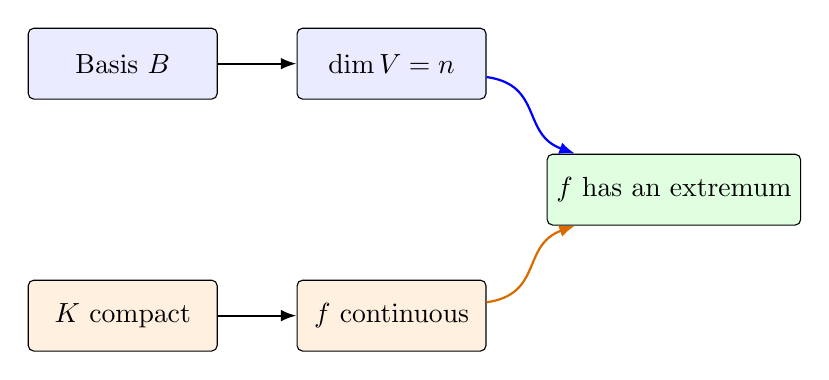
\begin{tikzpicture}[
  start chain=algebra going right,
  start chain=analysis going right,
  start chain=theorem going right,
  fact/.style={
    draw,
    rounded corners=2pt,
    minimum width=24mm,
    minimum height=9mm,
    align=center
  },
  every join/.style={-{Latex[length=2mm]},thick}
]
  \node[fact,on chain=algebra,fill=blue!8] (basis) at (0,1.6) {Basis $B$};
  \node[fact,on chain=algebra,fill=blue!8] (dimension) {$\dim V=n$};

  \node[fact,on chain=analysis,fill=orange!12] (compact) at (0,-1.6) {$K$ compact};
  \node[fact,on chain=analysis,fill=orange!12] (continuous) {$f$ continuous};

  \node[
    fact,
    on chain=theorem,
    fill=green!12,
    join=with algebra-end by {blue,out=-8,in=160,looseness=1.25},
    join=with analysis-end by {orange!85!black,out=8,in=-160,looseness=1.25}
  ] (result) at (7,0) {$f$ has an extremum};

  \path[-{Latex[length=2mm]},thick]
    (basis) edge (dimension)
    (compact) edge (continuous);
\end{tikzpicture}
\end{document}
